\documentclass{report} 

\usepackage{graphicx}
\usepackage{float}
\usepackage{titlesec}
\usepackage{subcaption}
\usepackage{caption}
\usepackage[acronym]{glossaries}

\makeglossaries

% Number figures as <chapter>.<section>.<figure>
\renewcommand\thefigure{\thechapter.\thesection.\arabic{figure}}
\counterwithin{figure}{section}

\titlelabel{\thetitle.\quad}

\setlength{\parskip}{1em}
\setlength{\parindent}{0pt}


\begin{document}

\chapter*{List of Acronyms}
\addcontentsline{toc}{chapter}{List of Acronyms}

\begin{tabbing}

\hspace{2cm} \= \kill
AI \> Artificial Intelligence \\
COPD \> Chronic Obstructive Pulmonary Disease \\
COVID-19 \> Coronavirus Disease 2019 \\
CLAP \> Contrastive Learning Audio Processing \\
RAG \> Retrieval-Augmented Generation \\
LLM \> Large Language Model \\
CRISP-DM \> Cross-Industry Standard Process for Data Mining \\
RNN \> Recurrent Neural Network \\
CNN \> Convolutional Neural Network \\
DL \> Deep Learning \\
LlaMa \> Large Language Model Meta AI \\
BERT \> Bidirectional Encoder Representations from Transformers \\
BGE \> BERT Generated Embeddings \\
MRR \> Mean Reciprocal Rank \\
MAP \> Mean Average Precision \\
UCD \> User-Centered Design \\
BaaS \> Backend-as-a-Service \\
WHO \> World Health Organization \\
CDC \> Centers for Disease Control and Prevention \\
API \> Application Programming Interface \\
REST \> Representational State Transfer \\
UI \> User Interface \\
HTTPS \> Hypertext Transfer Protocol Secure \\
JSON \> JavaScript Object Notation \\
iOS \> iPhone Operating System \\
VS Code \> Visual Studio Code \\

\end{tabbing}


\newpage

\chapter*{General Introduction}
\addcontentsline{toc}{section}{General Introduction}

The rapid evolution of artificial intelligence (AI) and mobile technologies has brought transformative changes across multiple domains, including healthcare. These advancements are now enabling the design of intelligent systems that support early disease detection, remote monitoring, and accessible diagnostics. One area of growing relevance is respiratory health, particularly in light of the increased attention to respiratory diseases following the COVID-19 pandemic and the continued burden of chronic conditions such as asthma, chronic obstructive pulmonary disease (COPD), and sleep apnea.

Despite the prevalence of such conditions, access to timely and affordable respiratory screening remains limited in many parts of the world. Specialized medical equipment and trained professionals are often required to conduct auscultation and interpret respiratory anomalies. This reality poses a significant barrier to early detection and long-term monitoring—two factors that are critical to improving patient outcomes. The proliferation of smartphones, however, opens new opportunities for building accessible, AI-powered health tools that can reach broader populations.

This end-of-year project seeks to address this challenge by designing and implementing a mobile application capable of analyzing breathing sounds and providing AI-assisted respiratory diagnostics. The system enables users to record audio samples using a smartphone microphone, which are then processed using machine learning models trained to classify respiratory anomalies such as wheezing, crackles, and rhonchi. Based on the classification results, the system offers a preliminary diagnostic suggestion. To enhance usability and trust, a conversational AI assistant is also integrated—allowing users to ask questions, receive explanations, and obtain medically grounded feedback.

The core objective of the project is to provide a portable and intelligent solution for respiratory disease detection, one that combines ease of use, technical robustness, and medical relevance. Achieving this goal involves contributions across multiple areas of computer science, including mobile development, signal processing, deep learning, backend architecture, and natural language processing.

The mobile application is built using a cross-platform framework, ensuring compatibility with both Android and iOS devices. It includes modules for secure user authentication, audio recording, and diagnosis history tracking. The backend infrastructure, powered by a backend-as-a-service platform, supports encrypted data storage, API integration, and serverless functions for model inference. On the AI side, two main components are developed: (1) a contrastive learning model (CLAP) for respiratory sound classification, and (2) a lightweight retrieval-augmented generation (RAG) chatbot based on a quantized language model. These components are trained on publicly available datasets and fine-tuned to deliver fast, accurate, and explainable results to end users.

Beyond implementation, this report provides a structured exploration of the project lifecycle, from the initial definition of objectives to system evaluation. Chapter 1 introduces the general context, the underlying problem, and the proposed solution. Chapter 2 outlines the foundational concepts that support the system, including respiratory anomalies, deep learning principles, and mobile development strategies. Chapter 3 presents a review of related work in respiratory diagnostics and medical chatbots. Chapters 4 and 5 detail the application of the CRISP-DM methodology to both the classification model and the AI assistant. Chapter 6 focuses on implementation, highlighting system architecture, mobile development, backend integration, and the tools used.

Through this interdisciplinary work, we aim not only to demonstrate the feasibility of smartphone-based respiratory diagnostics, but also to contribute to the broader field of AI for public health. By combining modern machine learning techniques with accessible mobile interfaces, the project aspires to bring preliminary respiratory screening closer to users—anytime, anywhere.


\newpage

\setcounter{chapter}{2}  % Start from chapter 2
\setcounter{section}{0}
\chapter*{Chapter 2: Business Understanding and Key Concepts}
% intro + 2.1 + 2.2
\section{Mobile Development Concepts}
\label{sec:mobile_concepts}

Mobile development refers to the design and creation of software applications intended to operate on mobile devices such as smartphones and tablets. In the context of this project, mobile development serves as the foundation for the user-facing component of the system, enabling users to interact with diagnostic features, access results, and consult the AI assistant. This section introduces the key mobile development concepts relevant to the architecture used in this work.

\subsubsection*{Cross-Platform Development}

Cross-platform development is a software development approach that allows a single application codebase to be deployed on multiple operating systems, most notably Android and iOS. This reduces redundancy and development effort while maintaining consistency in functionality and design. It is especially beneficial in healthcare applications, where uniform user experience and rapid iteration are critical.

\subsubsection*{Modular Mobile Architecture}

A modular architecture divides the application into independent functional units, such as user interface components, business logic, and data services. This separation of concerns improves scalability, testability, and long-term maintainability. It also supports incremental feature integration—particularly important in complex systems like diagnostic platforms.

\subsubsection*{User-Centered Design in Health Applications}

Mobile health applications must prioritize accessibility, clarity, and ease of use. User-centered design (UCD) involves tailoring the interface to user needs, using intuitive navigation, medically neutral colors, and readable typography. These design principles are especially important in applications intended for patients, where cognitive load and clarity directly impact usability.

\subsubsection*{Data Privacy and Security Principles}

Mobile applications that handle health-related data must comply with strict privacy and security guidelines. Core concepts include local data encryption, secure authentication flows, permission-based access to device hardware (e.g., microphone), and encrypted communication channels. These safeguards help ensure that personal health information is protected throughout the diagnostic process.

\subsubsection*{Real-Time and Asynchronous Interaction}

Many mobile applications rely on real-time feedback and asynchronous operations—such as sending diagnostic data to a server and waiting for results. Concepts such as event-driven programming, state management, and asynchronous networking are fundamental to building responsive, interactive experiences without blocking the user interface.

\subsubsection*{Summary}

This section introduced the theoretical foundations of mobile development as they apply to healthcare systems. Concepts such as cross-platform development, modular architecture, security, and user-centered design provide the groundwork for implementing reliable and accessible diagnostic tools on mobile platforms. These principles informed the design decisions detailed later in the implementation chapter.

\section*{Conclusion}
\addcontentsline{toc}{section}{Conclusion}

\label{sec:chapter2_conclusion}

This chapter introduced the key domains that underpin the design of our AI-powered respiratory diagnosis system. These domains—medical anomalies, deep learning, and mobile development—serve as the conceptual foundation for the project's implementation.

First, we explored the nature of respiratory anomalies and their clinical significance, highlighting sounds such as wheezing, crackles, and stridor. These sounds provide early indicators of diseases like asthma, pneumonia, and COPD. Understanding their acoustic characteristics is essential for developing diagnostic algorithms that can detect them automatically.

Second, we reviewed core deep learning concepts, with a focus on audio classification using models such as CLAP, as well as the use of large language models (LLMs) for natural language understanding. These AI tools enable the system to both analyze user-recorded audio and provide conversational explanations and guidance through the integrated assistant.

Finally, we presented key mobile development concepts relevant to our implementation. Cross-platform development, modular architecture, responsive design, and data privacy principles ensure that the system remains accessible, secure, and user-friendly across devices. These concepts support the delivery of accurate, real-time diagnostics directly through a mobile interface.

Together, these foundations—clinical, algorithmic, and technical—set the stage for the practical implementation of our system, detailed in the chapters that follow.


\newpage

\setcounter{chapter}{6}  % Start from chapter 6
\setcounter{section}{0}
\chapter*{Chapter 6: Implementation}


\section*{Introduction}
\addcontentsline{toc}{section}{Introduction}

This chapter presents the implementation phase of our project: an AI-powered mobile application designed to analyze breathing sounds and assist in detecting respiratory diseases.

The implementation phase translates theoretical concepts into a working system. It focuses on the tools, technologies, and methodologies used to build the application and ensure its reliability and performance.

The core objective is to develop a mobile app capable of recording respiratory audio, uploading it securely, and using AI-based models to provide preliminary diagnostic feedback. The app also allows users to upload medical reports and offers a simple, intuitive interface with real-time insights.

To achieve this, we adopted a modular architecture that separates mobile development, backend services, and AI inference. The mobile app was developed using Flutter, chosen for its cross-platform capabilities and development speed. Appwrite was selected as the backend platform for its support of authentication, storage, and serverless functions.

This chapter begins with an overview of the system architecture and its components. It then details the implementation of key modules, including audio capture and encryption, data transmission, backend integration, and AI model deployment. Each section highlights the technical decisions made and the reasoning behind them.

\section{System Architecture}
\label{sec:system_architecture}

The system architecture of our AI-powered mobile application is designed to ensure modularity, scalability, and secure data handling. It is composed of three main components: the mobile application, the backend services, and the AI inference engine. Each component plays a distinct role while communicating seamlessly with the others.

The architecture follows a modular pattern to facilitate independent development and testing of each module. This design choice improves maintainability and simplifies the integration of additional features in the future.

The overall system structure is illustrated in Figure~\ref{fig:system-architecture}, which outlines the interactions between the core components of the application.


\begin{figure}[H]
    \centering
    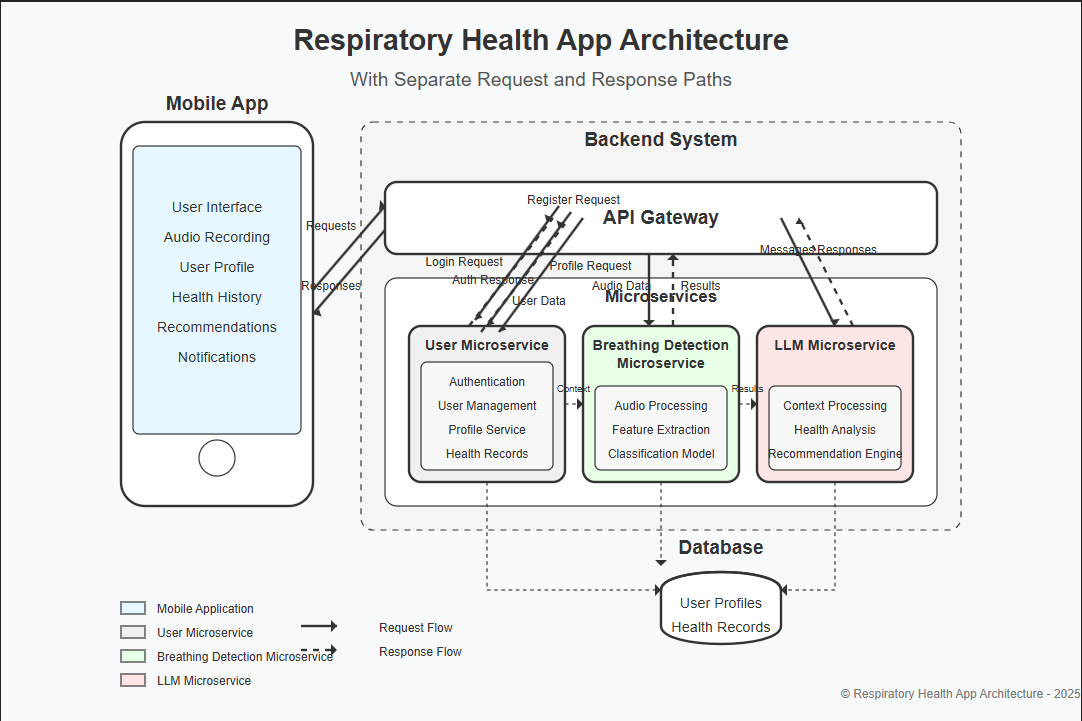
\includegraphics[width=\textwidth]{images/architecture.png}
    \caption{System Architecture of the AI-Powered Mobile Application}
    \label{fig:system-architecture}
\end{figure}

\subsubsection*{Mobile Application}

The mobile application, developed using Flutter, provides the user interface and handles client-side functionalities. These include audio recording, local encryption, file selection, and UI interactions. It also manages authentication and communication with the backend.

\subsubsection*{Backend Services}

The backend is powered by Appwrite, a self-hosted backend-as-a-service platform. It handles authentication, file storage (medical reports and audio), and serverless functions. Appwrite ensures secure and scalable data management while offering APIs that are easy to integrate with Flutter.

\subsubsection*{AI Inference Engine}

The AI inference module is responsible for analyzing respiratory audio data and generating preliminary diagnostic feedback. Once an audio file is uploaded and validated, it is sent to a dedicated inference server or function that runs a pre-trained deep learning model to detect anomalies in the breathing pattern.

\vspace{1em}

This modular architecture enables efficient development, enhances security, and supports the core functionality of respiratory disease detection.

\section{Mobile Application}
\label{sec:mobile_application}

The mobile application serves as the central user interface of our AI-powered respiratory analysis system. Built with Flutter, it offers a seamless and cross-platform experience. This section presents a walkthrough of the app’s core features, showcasing its design, functionality, and user flow.

\subsection{Visual Identity and Design Language}

The application embraces a medically inspired color palette referencing the official World Health Organization (WHO) guidelines, aiming for clarity, trust, and accessibility. The logo symbolizes the lungs through a stylized graphic, while the central dot represents a sensor tasked with detecting respiratory anomalies.

The primary branding elements, including both filled and outline logo variants, are shown in Figure~\ref{fig:app_logos}.

\begin{figure}[H]
    \centering
    
\includegraphics[width=0.25\textwidth]{images/UI_Screenshots/logo_filled.png}
    \hspace{2em}
    
\includegraphics[width=0.25\textwidth]{images/UI_Screenshots/logo_unfilled.png}
    \caption{Application Logos: Filled and Outline}
    \label{fig:app_logos}
\end{figure}

\subsection{Authentication: Login and Signup}

The user journey begins with secure authentication. A simple interface for logging in or signing up is provided, as seen in Figure~\ref{fig:login_screen}.

\begin{figure}[H]
    \centering
    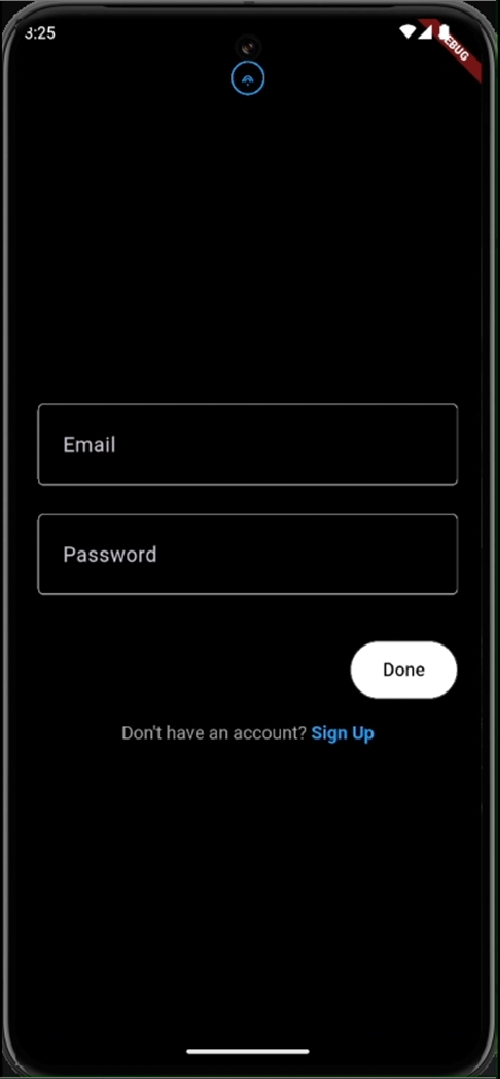
\includegraphics[width=0.35\textwidth]{images/UI_Screenshots/login_screen.png}
    \caption{Login Screen}
    \label{fig:login_screen}
\end{figure}

\subsection{User Profile Management}

Once authenticated, users are directed to a profile screen where they can view and manage their personal information. This interface is illustrated in Figure~\ref{fig:profile_screen}.

\begin{figure}[H]
    \centering
    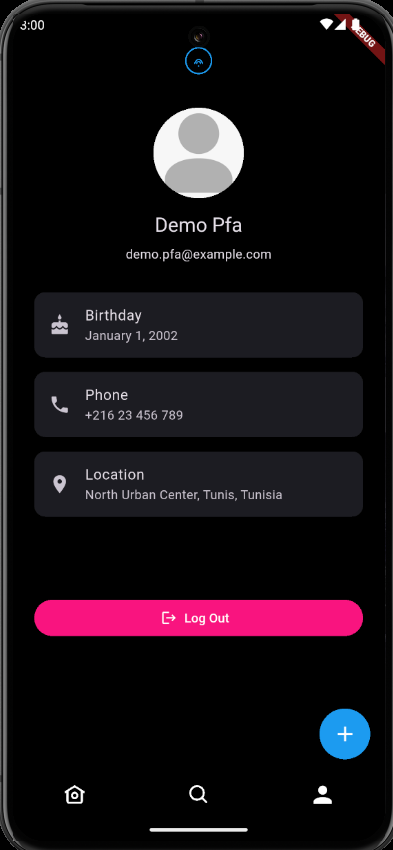
\includegraphics[width=0.35\textwidth]{images/UI_Screenshots/profile_screen.png}
    \caption{Profile Screen}
    \label{fig:profile_screen}
\end{figure}

\subsection{Home Screen – No Diagnoses Yet}

The initial home screen is presented when the user has not yet submitted any diagnoses. This clean interface is displayed in Figure~\ref{fig:home_screen_empty}.

\begin{figure}[H]
    \centering
    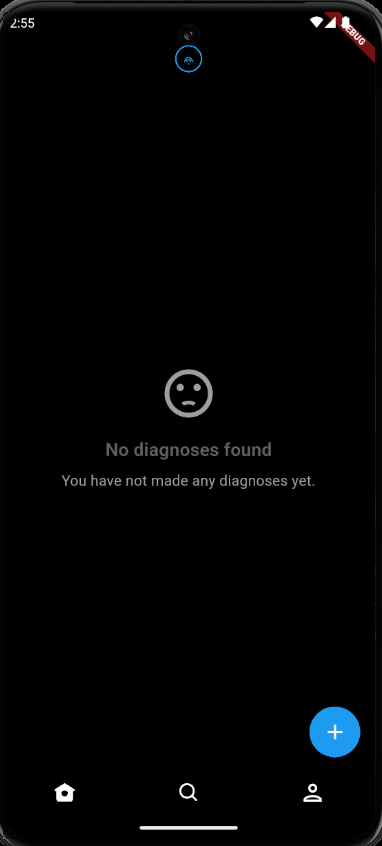
\includegraphics[width=0.35\textwidth]{images/UI_Screenshots/home_screen_no_diagnoses.png}
    \caption{Home Screen Without Diagnoses}
    \label{fig:home_screen_empty}
\end{figure}

\subsection{Search Screen – No History}

A search feature is available for reviewing past diagnoses. In the absence of history, the interface appears as shown in Figure~\ref{fig:search_screen_empty}.

\begin{figure}[H]
    \centering
    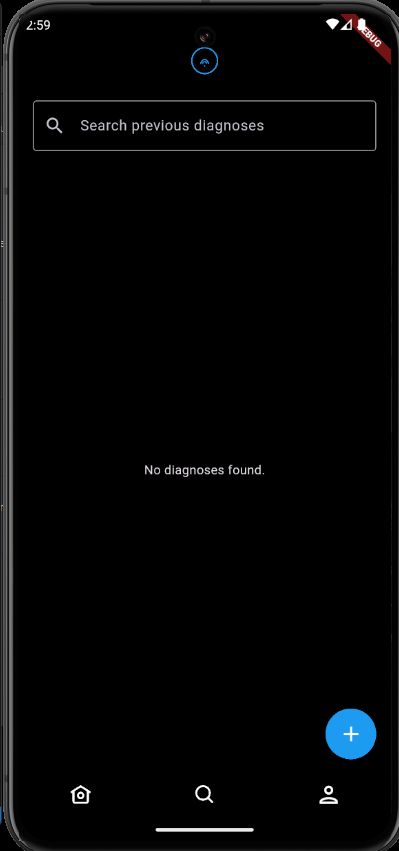
\includegraphics[width=0.35\textwidth]{images/UI_Screenshots/search_screen.png}
    \caption{Search Screen Without History}
    \label{fig:search_screen_empty}
\end{figure}

\subsection{Creating a New Diagnosis}

To start a diagnosis, users can record audio, upload medical files, and input symptoms using the interface shown in Figure~\ref{fig:create_diagnosis}.

\begin{figure}[H]
    \centering
    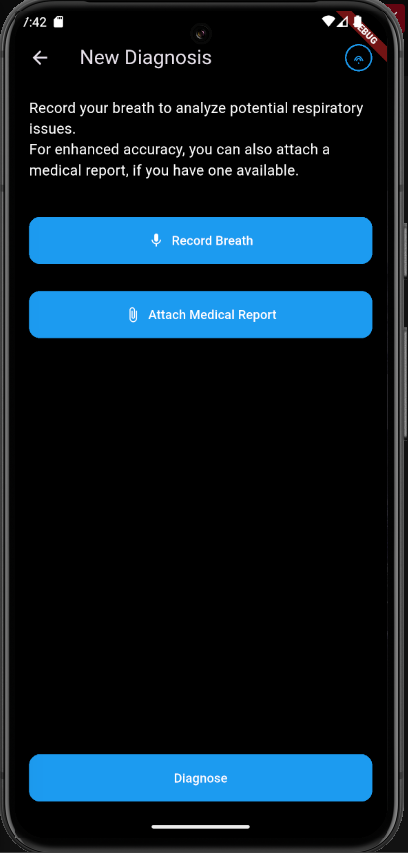
\includegraphics[width=0.35\textwidth]{images/UI_Screenshots/create_diagnosis_screen.png}
    \caption{Diagnosis Creation Interface}
    \label{fig:create_diagnosis}
\end{figure}

\subsection{Home Screen – With Previous Diagnoses}

After a diagnosis is performed, the home screen updates to reflect the user's diagnostic history, as demonstrated in Figure~\ref{fig:home_screen_with_history}.

\begin{figure}[H]
    \centering
    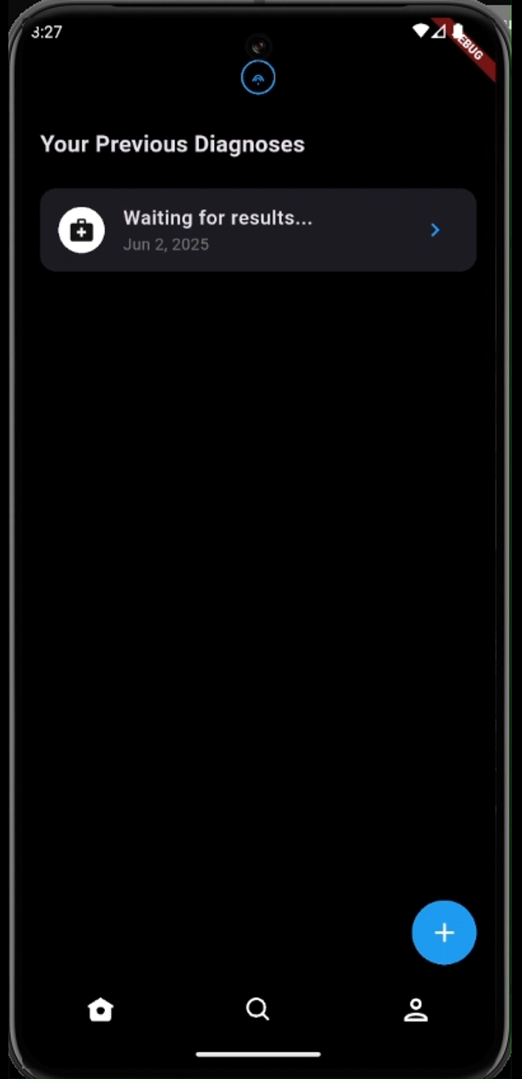
\includegraphics[width=0.35\textwidth]{images/UI_Screenshots/home_screen_with_previous_diagnoses.png}
    \caption{Home Screen Displaying Previous Diagnoses}
    \label{fig:home_screen_with_history}
\end{figure}

\subsection{Diagnosis Details – Waiting for Results}

Once a new diagnosis is submitted, the system informs the user that the analysis is in progress. This intermediate state is depicted in Figure~\ref{fig:diagnosis_waiting}.

\begin{figure}[H]
    \centering
    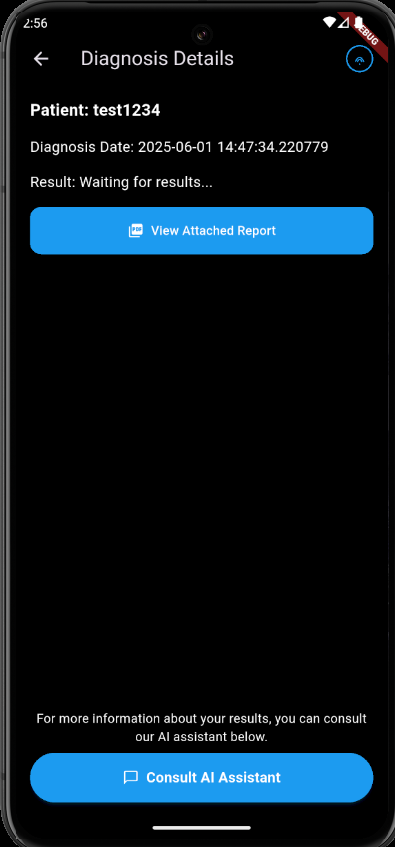
\includegraphics[width=0.35\textwidth]{images/UI_Screenshots/diagnosis_details_screen_waiting_for_results.png}
    \caption{Diagnosis Details – Awaiting AI Analysis}
    \label{fig:diagnosis_waiting}
\end{figure}

\subsection{Diagnosis Details – Results Ready}

After analysis is complete, users are presented with detailed diagnostic feedback, as shown in Figure~\ref{fig:diagnosis_results}.

\begin{figure}[H]
    \centering
    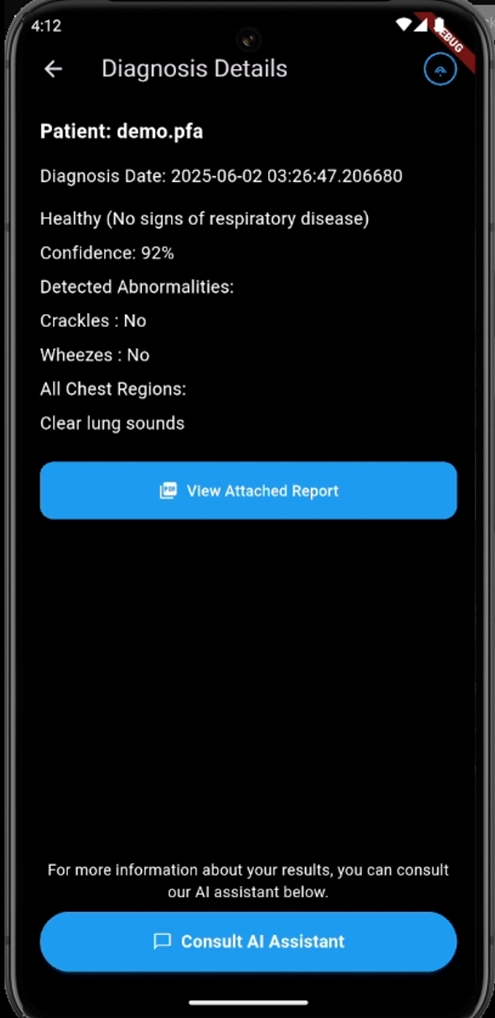
\includegraphics[width=0.35\textwidth]{images/UI_Screenshots/diagnosis_details_screen_results_ready.png}
    \caption{Diagnosis Details – Results Ready}
    \label{fig:diagnosis_results}
\end{figure}

\subsection{AI Assistant Onboarding}

When consulting the AI assistant for the first time, users are guided through an onboarding screen that outlines its purpose, as illustrated in Figure~\ref{fig:ai_onboarding}.

\begin{figure}[H]
    \centering
    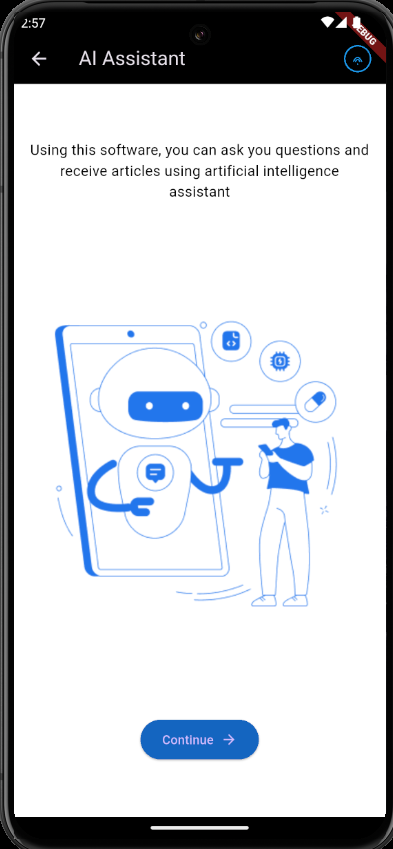
\includegraphics[width=0.35\textwidth]{images/UI_Screenshots/on_boarding_ai_assistant_screen.png}
    \caption{AI Assistant Onboarding Screen}
    \label{fig:ai_onboarding}
\end{figure}

\subsection{AI Assistant – Start Screen}

Following onboarding, users arrive at a starting interface that invites medical queries, as depicted in Figure~\ref{fig:ai_start}.

\begin{figure}[H]
    \centering
    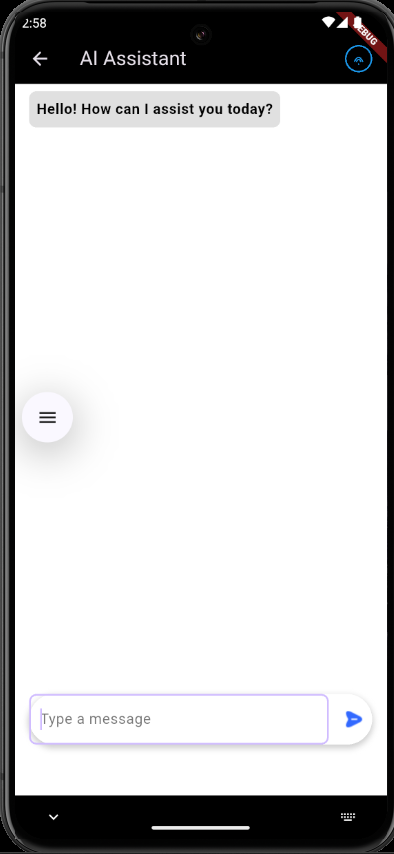
\includegraphics[width=0.35\textwidth]{images/UI_Screenshots/ai_assistant_screen_starting_screen.png}
    \caption{AI Assistant – Starting Interface}
    \label{fig:ai_start}
\end{figure}

\subsection{AI Assistant – Chat Interface}

The assistant responds in a conversational style, as shown in Figure~\ref{fig:ai_chat}, providing interactive, medically grounded guidance.

\begin{figure}[H]
    \centering
    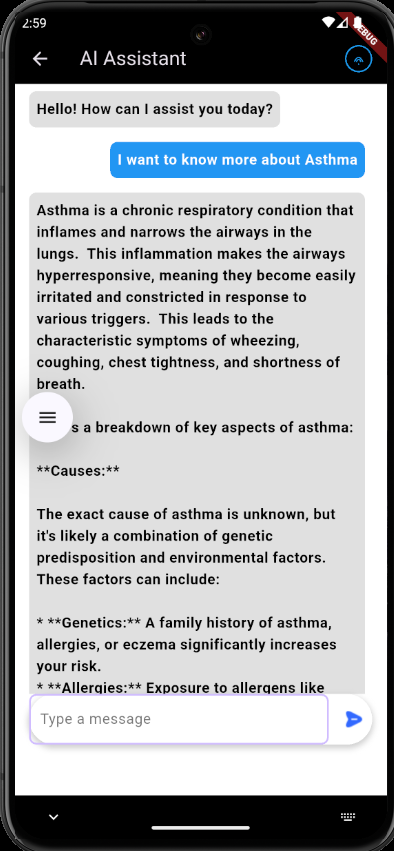
\includegraphics[width=0.35\textwidth]{images/UI_Screenshots/ai_assistant_screen_chat_example.png}
    \caption{AI Assistant Chat Interaction}
    \label{fig:ai_chat}
\end{figure}

\subsection{Summary}

The mobile application was designed to deliver a smooth, medically reliable, and user-centric experience. Each screen plays a specific role in guiding the user through authentication, diagnosis creation, result review, and AI consultation. Leveraging Flutter, the app ensures cross-platform consistency and accessibility. The clear design, inspired by WHO standards, and the integration of visual cues like the lung-symbol logo reinforce its identity as a trusted respiratory health tool.

\newpage

\section{Backend and API Integration}
\label{sec:backend_api}

The backend infrastructure is a critical component of our AI-powered mobile application, enabling secure data handling, user management, and seamless communication between the mobile client and AI services. Built around Appwrite—a self-hosted backend-as-a-service (BaaS) platform—the system benefits from a robust, modular, and scalable architecture.

\subsection{Appwrite as Backend-as-a-Service (BaaS)}

Appwrite serves as the core backend platform, providing essential services such as authentication, database storage, file handling, serverless computing, and real-time updates. It supports structured data for user profiles and health records, encrypted storage for audio and medical files, and custom functions for executing AI-based health analysis.

The architecture shown in Figure~\ref{fig:appwrite_backend} depicts how the Flutter-based mobile frontend communicates with Appwrite services over secure HTTPS, enabling a seamless flow of authentication, data storage, and diagnostic processing. Each backend service operates independently while being orchestrated via the Appwrite API Gateway, which manages routing and authentication for all client requests.

\begin{figure}[H]
    \centering
    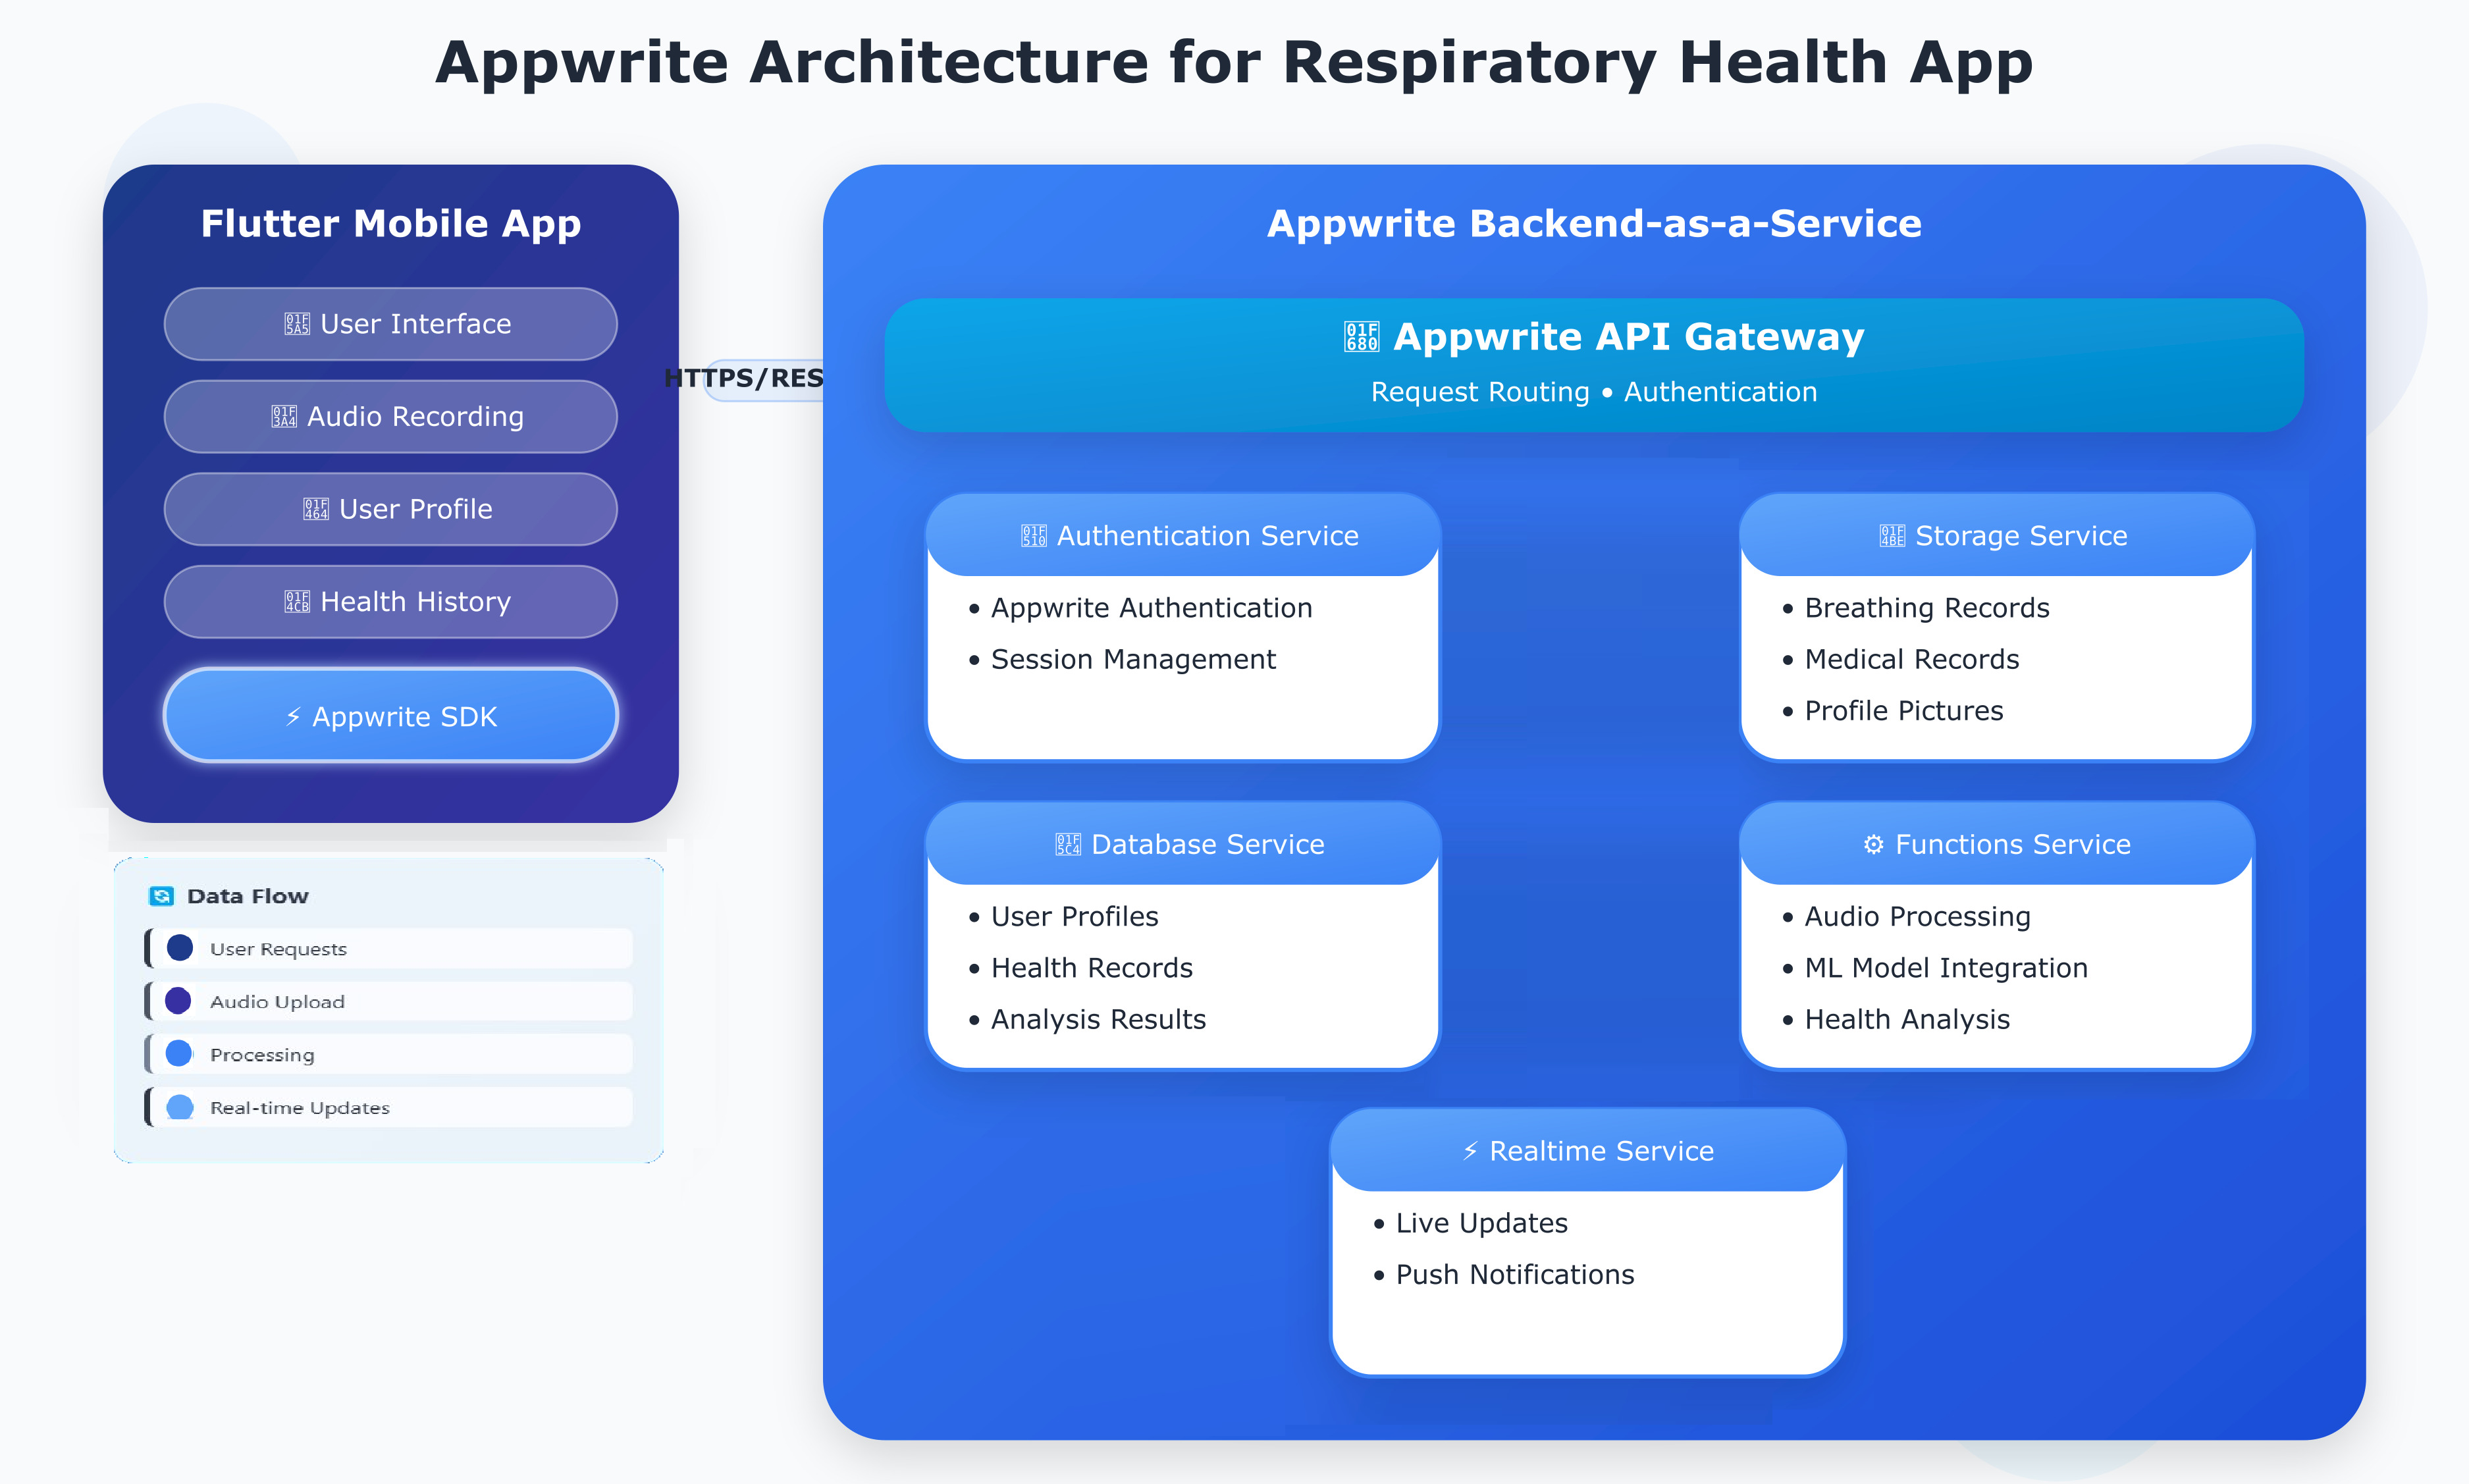
\includegraphics[width=0.95\textwidth]{images/backend/apprwite_architecture.png}
    \caption{Appwrite-Based Backend Architecture}
    \label{fig:appwrite_backend}
\end{figure}

\subsection{Authentication and Session Management}

User authentication is handled through Appwrite’s secure email-password mechanism. Upon successful login or registration, the client receives a session token, which is used to authorize all subsequent requests. This approach ensures privacy, data isolation, and secure access to personalized health information.

\subsection{Diagnosis Submission and File Handling}

When a user initiates a new diagnosis, the application uploads the audio recording and any supplementary files to Appwrite’s storage service. These assets are then linked to a new diagnosis document in the Appwrite database, which contains relevant metadata such as the timestamp, reported symptoms, and user ID.

\subsection{Triggering AI Inference}

Following submission, an Appwrite function is triggered asynchronously. This serverless function retrieves the uploaded audio file, forwards it to the AI inference engine through a secure REST API, and receives a structured JSON response. The results—comprising predicted conditions, confidence scores, and supplementary data—are saved back to the corresponding document in the database.

\subsection{Result Synchronization with the Mobile App}

To ensure responsiveness, the mobile app routinely polls the backend for updates to diagnosis records. When inference results are available, the interface updates to reflect the final diagnosis. Optionally, Appwrite’s real-time services can push changes to the client directly, allowing live updates and improved interactivity in future versions.

\subsection{Summary}

The backend architecture effectively bridges the user-facing application with the AI-driven analysis pipeline. Appwrite provides a secure, modular environment for managing identity, health data, and inference workflows. This integration enables scalable diagnostics while maintaining user privacy and system extensibility.

\section{Tools and Technologies Used}  
\label{sec:tools_tech}

The development of our AI-powered mobile diagnostic system was supported by a carefully selected suite of tools, frameworks, and platforms that together ensured efficiency, scalability, and security across the entire stack. This section introduces the core technologies employed throughout the project.

\subsection{Flutter for Cross-Platform Development}

Flutter was chosen as the core framework for building the mobile application, enabling a unified codebase for both Android and iOS platforms. Its declarative UI toolkit and reactive architecture allowed for efficient development and a smooth user experience.

The Flutter logo is shown in Figure~\ref{fig:flutter_logo}.

\begin{figure}[H]
    \centering
    
\includegraphics[width=0.25\textwidth]{images/tools/flutter.png}
    \caption{Flutter Logo}
    \label{fig:flutter_logo}
\end{figure}

\subsection{Dart Programming Language}

Dart, the language behind Flutter, was used for implementing both application logic and UI elements. Its type safety and support for asynchronous operations made it well-suited for responsive mobile development.

The Dart logo is displayed in Figure~\ref{fig:dart_logo}.

\begin{figure}[H]
    \centering
    
\includegraphics[width=0.2\textwidth]{images/tools/dart.png}
    \caption{Dart Logo}
    \label{fig:dart_logo}
\end{figure}

\subsection{Appwrite for Backend-as-a-Service}

Appwrite was selected as the backend-as-a-service solution, offering user authentication, database storage, file handling, and serverless functions. Its modular design simplified backend operations and enhanced security.

The Appwrite logo is presented in Figure~\ref{fig:appwrite_logo}.

\begin{figure}[H]
    \centering
    
\includegraphics[width=0.3\textwidth]{images/tools/appwrite.png}
    \caption{Appwrite Logo}
    \label{fig:appwrite_logo}
\end{figure}

\subsection{Python for AI Model Deployment}

Python was used to develop and deploy the AI inference engine, leveraging libraries such as PyTorch and Hugging Face Transformers for audio-based diagnosis prediction.

The Python logo can be seen in Figure~\ref{fig:python_logo}.

\begin{figure}[H]
    \centering
    
\includegraphics[width=0.25\textwidth]{images/tools/python.png}
    \caption{Python Logo}
    \label{fig:python_logo}
\end{figure}

\subsection{REST APIs for Communication}

RESTful APIs facilitated communication between the mobile frontend, Appwrite backend, and AI inference engine. This decoupled architecture allowed independent scaling and streamlined integration.

A representation of REST APIs is shown in Figure~\ref{fig:restapi_logo}.

\begin{figure}[H]
    \centering
    
\includegraphics[width=0.2\textwidth]{images/tools/restapi.png}
    \caption{REST API Representation}
    \label{fig:restapi_logo}
\end{figure}

\subsection{Docker for Containerization}

Docker was employed to containerize both Appwrite services and the AI backend. This ensured consistent deployment, streamlined development, and enhanced scalability.

The Docker logo is illustrated in Figure~\ref{fig:docker_logo}.

\begin{figure}[H]
    \centering
    
\includegraphics[width=0.3\textwidth]{images/tools/docker.png}
    \caption{Docker Logo}
    \label{fig:docker_logo}
\end{figure}

\subsection{VS Code and Postman for Development and Testing}

Visual Studio Code served as the primary development environment, providing extensive support for Dart, Flutter, and Python development.

The VS Code logo is shown in Figure~\ref{fig:vscode_logo}.

\begin{figure}[H]
    \centering
    
\includegraphics[width=0.2\textwidth]{images/tools/vscode.png}
    \caption{VS Code Logo}
    \label{fig:vscode_logo}
\end{figure}

Postman was used for testing API endpoints and simulating request flows during diagnosis.

The Postman logo is displayed in Figure~\ref{fig:postman_logo}.

\begin{figure}[H]
    \centering
    
\includegraphics[width=0.2\textwidth]{images/tools/postman.png}
    \caption{Postman Logo}
    \label{fig:postman_logo}
\end{figure}

\subsection{Android Studio for Android Emulation}

Android Studio was utilized to run the Android emulator, enabling thorough testing of the mobile application on virtual Android devices and ensuring compatibility and performance.

The Android Studio logo is shown in Figure~\ref{fig:androidstudio_logo}.

\begin{figure}[H]
    \centering
    
\includegraphics[width=0.25\textwidth]{images/tools/androidstudio.png}
    \caption{Android Studio Logo}
    \label{fig:androidstudio_logo}
\end{figure}

\subsection{Git and GitHub for Version Control}

Version control was managed using Git, with GitHub as the remote repository. This setup supported collaborative development, issue tracking, and code versioning.

The Git and GitHub logos are presented in Figure~\ref{fig:git_github_logo}.

\begin{figure}[H]
    \centering
    
\includegraphics[width=0.4\textwidth]{images/tools/git_github.png}
    \caption{Git and GitHub Logos}
    \label{fig:git_github_logo}
\end{figure}

\subsection{Summary}

The integration of these technologies ensured a robust, maintainable, and scalable solution. From frontend development to AI inference and deployment, each tool played a critical role in delivering a reliable diagnostic experience to end users.

\newpage


\section*{Conclusion}
\addcontentsline{toc}{section}{Conclusion}

\label{sec:system_summary}

This chapter provided a comprehensive overview of the system architecture and implementation details of the AI-powered mobile diagnosis application. The system is structured into three main layers: the mobile frontend, the backend infrastructure, and the AI inference engine. Each component was designed to support secure, efficient, and scalable workflows for users seeking preliminary medical feedback.

The mobile application, developed using Flutter, offers a cross-platform interface for users to describe symptoms and receive AI-generated diagnostic results. Its intuitive design and responsive UI enhance user engagement and streamline the diagnosis submission process.

The backend, powered by Appwrite, handles authentication, data storage, and serverless function execution. It acts as a secure intermediary between the mobile client and the AI inference engine, ensuring encrypted data handling, user-specific data isolation, and real-time result synchronization.

The AI pipeline, built using Python and transformer-based models, interprets audio symptom descriptions and returns structured diagnostic suggestions. It integrates seamlessly with the backend via REST APIs, enabling efficient model inference workflows.

Together, these components form a robust, modular architecture that supports accurate, secure, and real-time delivery of diagnostic information. The technology stack and integration strategy ensure future scalability, maintainability, and adaptability to more advanced diagnostic features.


\newpage

\chapter*{General Conclusion}
\chapter*{Conclusion and Perspectives}
\addcontentsline{toc}{chapter}{Conclusion and Perspectives}
\rhead{Conclusion and Perspectives}

\section*{Conclusion}

This project presented the design and implementation of an AI-powered mobile application for breathing analysis and the detection of respiratory anomalies. The system combines mobile development with advanced AI techniques to deliver a modern, accessible diagnostic tool that supports early screening for conditions such as asthma, pneumonia, COPD, and sleep apnea.

The application allows users to record their breathing sounds, upload medical reports, and interact with an AI assistant. Through the use of Flutter for frontend development and Appwrite as a secure backend platform, the system ensures a smooth, cross-platform experience while maintaining user privacy and data integrity. On the AI side, the pipeline includes respiratory sound classification using deep learning models and personalized feedback powered by large language models (LLMs), enabling both automated diagnosis and natural language interaction.

The modular system architecture, built around RESTful APIs and containerized services, enabled seamless integration between the frontend, backend, and AI components. Tools like Docker, Git, Postman, and VS Code contributed to a robust and maintainable development workflow.

\section*{Perspectives}

While the current version of the application demonstrates the feasibility and effectiveness of AI-assisted respiratory analysis, several avenues remain for future improvement:

\begin{itemize}
  \item \textbf{Improved Audio Processing:} Incorporating advanced audio enhancement techniques, such as adaptive noise cancellation and real-time denoising, would increase the robustness of predictions in noisy environments.
  
  \item \textbf{Model Optimization and On-Device Inference:} Future iterations could explore model compression and quantization techniques to allow inference directly on the mobile device, improving response time and reducing backend dependency.

  \item \textbf{Dataset Expansion:} Increasing the diversity and size of the training dataset — including data from various age groups, devices, and environments — would improve the model’s generalization to real-world scenarios.

  \item \textbf{User Feedback Integration:} Allowing users to provide structured feedback on the accuracy of diagnoses and AI assistant responses could help continuously refine the system.

  \item \textbf{Medical Integration:} Long-term perspectives include integration with clinical workflows or partnerships with healthcare providers to support telehealth and digital triage systems.

  \item \textbf{Security and Regulatory Compliance:} Future versions should consider compliance with medical data regulations (e.g., GDPR, HIPAA) and formal security audits to ensure safe deployment in healthcare settings.
\end{itemize}

In conclusion, this project highlights the potential of combining mobile technologies with AI to support respiratory healthcare. With continued development and validation, this system can evolve into a trusted tool for early screening, patient monitoring, and AI-powered clinical assistance.





\end{document}
